\chapter{Introduction}

In recent decades, the global flow of Foreign Direct Investment (FDI) has
steadily increased, rising from almost nothing in the 1970s to over \$2.3
trillion dollars in 2016, becoming an important source of global capital. For
developing countries especially, capital from Multinational Corporations (MNCs) is robust to
global economic downturns, prompting major international
organizations to endorse FDI as a key factor to economic development and poverty reduction
(Figure~\ref{fig:globalfdi}) \citep{Mallampally1999, WorldEconomicForum2013}.
Within the International Political Economy
(IPE),  much of the literature also starts with the view that FDI bring various
benefits to the host countries, and that these countries will always seek FDI \citep{Jensen2008b}. These works focus on \textit{how} countries can attract FDI, and do
not question \textit{whether} they want to do so \citep{Jensen2003, Li2003, Li2006,
  Ahlquist2006}.\footnote{Two recent exceptions are \citet{Pinto2013,
    Pandya2016}, which are the first to examine countries' demand for FDI.} 

\begin{figure}[tbp]
  \centering
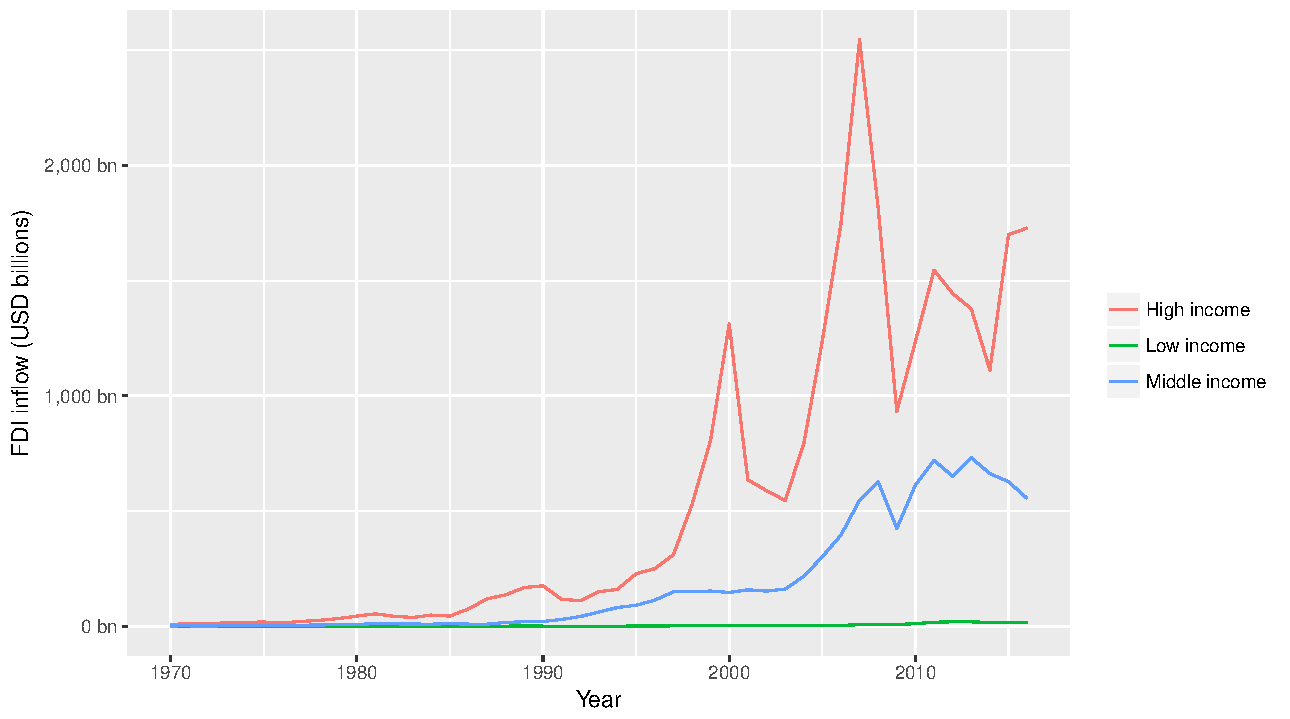
\includegraphics[width=0.8\textwidth,keepaspectratio]{../figure/global_fdi}
\caption[FDI global inflow, 1970-2006.]{FDI global inflow, 1970-2006. The last
  four decades witness the growth of FDI into the most important
  source of global capital. Source: World Bank's World Development Indicators.}
\label{fig:globalfdi}
\end{figure}

At first glance, the benefits of FDI do not seem controversial. In addition to bringing capital to and creating jobs in the host economy, FDI
holds an important promise that is the spillover of productivity from foreign to
domestic firms. As well-known from neoclassical growth theory, diminishing
returns to capital will at one point stop capital from accumulating further,
preventing long-run economic growth from being driven by capital accumulation
alone \citep{Solow1956}. \citet{Findlay1978}'s groundbreaking model of FDI and
growth shows how FDI can counteract this dynamics. In this model, technology spillover from foreign firms shift the domestic
factor-price frontier to the right, allowing more output from the same input,
ultimately resulting in a continually increasing capital stock for the domestic
sector. In this view, FDI is welfare-enhancing, providing spillover benefits to
local firms in ways that foreign firms do not take into account in their private
calculations. This claim about the positive effect
of FDI provides a justification for countries' using investment promotion to
rectify the ``undersupply'' of FDI \citep{Moran1998}. 

Despite this prevailing theoretical argument, recent empirical evidence shows
that not all FDI are the same and that its effects are highly conditional. There is no conclusive evidence of FDI having a positive effect on
growth \citep{Nair-Reichert2001, Carkovic2002} or poverty reduction
\citep{Guerra2009}. This puzzle opens a substantial literature on how the
growth-enhancing and spillover effect of FDI is conditional on the absorptive
capacity of the host economies, i.e. its level of human capital, technological
sophistication, and financial market development \citep{Durham2004,
  Nunnenkamp2004, Fu2008, Willem2004}. In addition, while the capital brought
and jobs created by FDI are unconditionally good for the overall economy, its
distributional effects across different constituencies in the host economy,
creating political cleavage across both sectoral and geographical divides
\citep{Chintrakarn2012, Goldberg2007, Nunnenkamp2007}.

Given the recent evidence on the conditional effect of FDI, it is no longer
tenable to hold the assumption that countries' preference for FDI is largely
homogeneous. By holding this assumption, we neglect the role of the
state in shaping global capital flow, falling prey to the discredited
``race to the bottom'' thesis of globalization \citep{Mosley2005}. Arguably,
examining countries' preference for FDI should be of more interest to political
scientists than the current focus on MNCs' location preference, which
often amounts to adding a political variable to an existing economic model of
FDI flow. Plus, even if we only care about MNCs' location preference, we must
still take into account countries' preference in order to get an accurate
estimate. For example, consider
the received wisdom that democracies receive more FDI \citep{Jensen2008a}.
Without controlling for countries' preferences, it is difficult to interpret this fact as
democracies actively pursuing MNCs or as MNCs finding democracies attractive.

\section{Goal of the Dissertation}

In essence, this dissertation aims to estimate the preference of both countries
and MNCs for each other. It develops an empirical strategy that takes into
account the two-sided nature of the FDI market, i.e. a FDI project can only
exist if both the MNC and the host country agree. Recognizing that this
two-sided matching dynamics can also be found in the labor or the marriage
markets, I adapt the statistical models first developed in Sociology for these
markets and apply them to the study of FDI \citep{Logan1996, Logan2008}.

In doing so, I simultaneously addresses three long-standing issues in the FDI literature.

First, I bring the state back in, filling the current gap in the literature on
the variation of countries' preference for FDI. Two notable exceptions are
\citet{Pinto2013} and \citet{Pandya2016}, whose pioneering works propose partisan politics
and regime types as factors shaping preferences for FDI. However,
while their theories are ground-breaking, the empirical estimation of countries'
preferences remains inadequate. In addition, these researchers have not
used their findings to re-estimate the preference of MNCs, separating out the
``push'' and ``pull'' factors of FDI flow.\footnote{``Push factors'' refer to
  characteristics of the home country and of the MNC, pushing capital out from its
  origin. ``Pull factors''
  refer to the characteristics of the host country, pulling capital towards its
  destination.} Using a two-sided matching model, I will naturally be able to
estimate both sides' preference.

Second, I propose that we need to theorize about countries' preferences for
different types of FDI. While the IPE literature has largely focused on the
quantity of FDI flows, national policies and discourses pay much attention to the quality of FDI, using various
incentives and restrictions to target certain types of FDI. Indeed, MNCs come
with varying amount of capital, labor demand, and technological sophistication,
all of which have different effects on the host country's economy. Just as the
two-sided matching model can estimate MNCs' utility functions for countries'
characteristics (e.g. market size, level of development), it can also estimate
countries' utility functions for MNCs' characteristics (e.g. technological
sophistication, export strategy).

Third, while the majority of the literature uses FDI stock
and flow data, these statistics are accounting constructs created to keep track
of countries' balance of payment and thus map poorly to concepts in Political
Science theories. Very often, the variable of interest in our theories is the scale of MNCs'
activities in the host country, which can be very different from the amount of
border-crossing capital thanks to MNCs' complex financial and tax strategies
\citep{Kerner2014}. Therefore, we would do much better testing our theories with
firm-level operational data. Unfortunately, even when firm-level FDI data is
available, the lack of a suitable statistical model poses a big barrier to this approach.

These three issues are related and represent the status quo in the FDI
literature. Data limitation forces scholars to look at country-level aggregate
FDI flow, making it difficult to study countries' preference for different types
of FDI. Without taking into account countries' preference, models of MNCs'
location choice are suspect.

In sum, my dissertation benefits the field by developing a empirical strategy that is capable of using firm-level data to estimate both firms' and countries' preferences for
each other's characteristics. To accomplish this goal, I adapt the two-sided
matching model originally designed for the labor market and the marriage market.
In this model, both MNCs and countries evaluate their available options
according to their utility functions, choose the best alternative, culminating
in a subsidiary being built by a MNC in a host country. Our goal is to estimate
MNCs' and countries' utility functions, and the challenge is to do so using only
data on which subsidiary is located where. Indeed, it would be straightforward
to estimate the utility functions if we observed not only the MNC's location decision
but also the set of options presented to the MNC.\footnote{Discrete choice
  models can be used to estimate the utility functions when both the choice and the set of options are observed.
  Indeed, this remains the dominant empirical approach in the industrial location
  literature, effectively ignoring the fact that not all firms have the same set
  of location options \citep{Arauzo-Carod2010}.} (Following the matching
literature, we call this set of options
the ``opportunity set.''). Unfortunately, while data on
subsidiaries' location are available, the opportunity set is generally
unobservable as researchers cannot peek into the negotiation process between
countries and MNCs. The two-sided matching model solves this problem by
using the Metropolis-Hastings algorithm, a Markov chain Monte Carlo (MCMC)
approach that repeatedly samples new opportunity sets and rejects them at an
appropriate rate to approximate their true distribution. Since the two-sided
matching model is derived explicitly from actors' utility functions, the
estimated parameters also have a convenient interpretation as the effect of different
variables on MNCs' and countries' utility. This allows us to make statements
such as ``in evaluating MNCs, China values a 2\% increase in the firm's capital as much as
a 1\% increase in labor demand.''

\section{Roadmap}

In the rest of this introductory chapter, I review in-depth the three issues in
the literature of FDI's political determinants, outlining the current attempts
to address them and how my approach can contribute to the solution.

In Chapter~\ref{chap:model}, I describe the two-sided matching model, including
both its game-theoretic origin and its statistical estimation.
Chapter~\ref{chap:simulation} uses simulations to demonstrate the correctness of
the model and explores its characteristics. Chapter~\ref{chap:labor} applies the
model on US labor market data, the original domain of the two-sided matching
approach, in order to compare with and expand upon previous results.
Chapter~\ref{chap:FDI} brings us back to the study of FDI, applying the model on
firm-level data of Japanese MNCs in East and Southeast Asia.
Chapter~\ref{chap:conclusion} concludes and explores potential applications of
the two-sided matching model in other areas of Political Science.

\section{Three Issues in the Literature of FDI's Political Determinants}
\label{sec:literature_issues}

\subsection{Measuring MNCs' Activities}

As \citet{Kerner2014} argues, the political economy literature on FDI is a bit
of a misnomer. Political scientists are rarely interested in FDI \textit{per
se}---rather, they are interested in the activities of MNCs, which in turn,
affect other important issues such as nation-state autonomy \citep{Mosley2005},
economic development \citep{Moran1998}, labor standards \citep{Mosley2007}, and
environmental policies \citep{Prakash2007}. However, while the theories involve
MNCs as the central actor in the causal mechanism, the empirics often use FDI
flow as the independent variable of interest. These two concepts---the level of
MNCs' affiliate activities in a country and FDI inflow into a country---are not
the same.

Consider the definition of FDI from UNCTAD, the main producer of FDI data widely
used by researchers:

\begin{quote} FDI has three components: equity capital, reinvested earnings and
intra-company loans.
\begin{itemize}
\item Equity capital, i.e. the foreign investor’s purchase of shares of an
enterprise [in the host country].
\item Reinvested earnings, i.e. the foreign investor’s share \ldots of earnings
not distributed as dividends by affiliates, or earnings not remitted to the
foreign investor.
  \item Intra-company loans between direct investors and affiliate enterprises.
\end{itemize} \citep[245]{UNCTAD2007}
\end{quote}

In essence, FDI data captures the amount of capital that crosses border. It is a
poor proxy for the scale of MNCs' activities in the host countries because it
overlooks important components of MNCs' activities while including components
that are only relevant for balance of payment statistics
\citep{Beugelsdijk2010}.

Consider the argument that FDI is the driver for the diffusion of labor
standards across countries. \citet{Mosley2007} theorizes that FDI can have this
effect through three channels. First, MNCs may pressure the host governments for
better rule of law and social programs. For MNCs to be able to effectively
pressure the host governments, they must prove themselves valuable to the
government by providing jobs or tax revenues. Both of these factors are only
tenuously related to the amount of foreign capital inside the host country.
Indeed, a MNC can employ thousands of employees, pay millions in tax, but show
up as a net 0 on FDI flow data because the profit is repatriated to the foreign
investor or through intra-company loans.\footnote{The issue of intra-company
loans is particularly fraught with issues because companies very frequently use
intra-company loans to get out of paying tax in a country. These loans will be
recorded on the book as a massive outflow, even though the MNC still has a large
presence on the ground.} The size of the MNCs' operation is further understated
because FDI statistics does not take into account capital raised locally. It
also does not take into account the productivity of MNCs, which acts as an
important multiplier when translating the amount of capital to the amount of
output.

Second, scholars argue that MNCs may bring along best practices for workers'
rights and spread it to local firms. If this channel operates via competition as
MNCs provide better working condition forcing local firms to compete, then MNCs
must employ a lot of labor for this effect to be noticeable. If this channel
operates via demonstration, then it must form a lot of linkages with local
firms, as suppliers and buyers, for the diffusion of norms to happen. Both the
size of the labor force and the type of linkages with the local economy are not
captured by FDI flow statistics.

Third, scholars argue MNCs may care more about labor quality than its cost, and
thus may invest in higher wages, better benefits, or more training. Once again,
for this effect to be noticeable, the size of the MNCs' labor force matters, its
industry, and its investment in productivity, matters a lot more than how much
capital it brings in and out of the country. In addition, non-equity
transactions between the foreign parent company and the local subsidiary are not
counted in FDI flow statistics, such as transfer of knowledge, technology, and
management practices, thus excluding a component that is arguably much more
important to labor quality than the amount of capital.\footnote{These issues are
not isolated to studies of FDI and labor standards, but are common to the whole
IPE literature of the effect of FDI on policy convergence, such as environmental
policies \citep{Prakash2007}.}

This mismatch may also be a reason behind the still unsettled debate on the
effect of FDI on poverty reduction. Scholars have theorized that FDI can lead to
economic development and through three channels. First, MNCs can simply provide
cheaper and better goods by being more productive. Second, MNCs may improve the
productivity of local economy through technology transfer. Finally, MNCs can
bring tax revenue to the host government, which can then spend on the poor via
investment into social programs. Once again, these causal mechanisms only work
depending the scale and the type of MNCs activities in the host country, not on
the amount of equity capital that crosses the border. For example, productivity
spillover is highly conditional on how thick the linkages between the MNCs and
the local suppliers are as well as how technologically advanced the MNCs'
activities are on the ground. The effect of FDI via tax revenue is particularly
fraught with issues, as MNCs frequently engage in transfer pricing to get out of
paying tax, especially via intra-company transactions of goods and services,
such as charging for internal IP, whose price can be set arbitrarily by the firm
\citep{Malesky2015c}, which are not recorded in FDI flow statistics, \footnote{A
similar argument is about the relationship of FDI on economic development,
especially on the technology spillover and tax revenue.}

What about studies that use FDI as the dependent variable, and are thus perhaps
interested in flow of capital in and of itself?\footnote{Arguably, political
scientists are not interested in the flow of capital in and of itself, but also
because of its implications for development, state autonomy, and other effects
on policy. The discussion above has shown how problematic it is to study these
effect of FDI using FDI flow data.} The vast majority of theories on the
political determinants of FDI flow relies on the ``obsolescing bargain'' model.
Originally developed by \citet{Vernon1971}, the model is so named because the
bargaining dynamics between the MNC and the host government changes over time,
initially favoring the MNC and gradually tips towards the host government as the
MNC commits more fixed capital on the ground. Indeed, knowing that it is costly
for the MNC to uproot its increasingly large and immobile operation, the host
government can unilaterally alter the original bargain, most egregiously by
expropriating the MNC's asset and profit, but more often via ``creeping
expropriation,'' e.g. increased tax or tougher regulation \citep{Li2009a}.
Political economists argue that MNCs are acutely aware of the ``obsolescing
bargain,'' and thus prefer to invest in countries whose governments can make a
credible commitment that they will not alter the original bargain. This means
MNCs prefer countries with democratic accountability \citep{Jensen2003}, a
federal system \citep{Jensen2005}, membership in international trade agreements
\citep{Buthe2008}, less political risk \citep{Beazer2011, Graham2010}, or more
veto points \citep{Choi2008}.\footnote{The fact that FDI is understood as
illiquid capital subject to the obsolescing bargain is the central theoretical
difference between FDI and footloose equity capital \citep{Ahlquist2006,
David2008}}.

The linchpin of this argument is the assumption that FDI capital is illiquid and
cannot be quickly removed from the host country at will. This assumption is not
fully warranted. According to the US Bureau of Economic Analysis (BEA)'s 2004
survey, 43\% of US MNCs' balance sheet comprises of liquid assets that can be
liquidated within one year under normal operating situations. Among the 57\% of
the balance sheet that are illiquid, 24\% are ``other non-current assets,''
which include non-tangible assets like brand names, trademarks, and
patents---some of which are not expected to be liquidated but can be removed
from the host countries. Only another 24\% of the balance sheet is made up of
physical capital, i.e. Plant, Property, and Equipment (PPE), which cannot be
easily moved and match most closely to what we have in mind as the ``illiquid
capital'' in the obsolescing bargain model \citep[113]{Kerner2014a}.

Besides the conceptual mismatch between FDI flow and MNCs' activities, from a
statistical standpoint, this measurement error may also be a contributing factor
to the still unsettled debate on the effect of FDI. Even when the measurement
error is random, it will inflates the standard error of our estimate when FDI is
the dependent variable, and bias our estimate towards 0 when FDI is the
independent variable. These effects may explain \citet{Jensen2012}'s surprising
finding that lower corporate tax rate does not lead to more FDI flow, or the
mixed empirical evidence for the relationship between FDI and development
\citep[108]{Mold2004}.

Even more worryingly, the measurement error is unlikely to be random. For
example, the amount of locally raised capital, something we care about but FDI
statistics does not capture, is likely to correlate with how developed the local
capital market or the fluctuation in the exchange rate. On the other hand,
repatriated earnings, something that does not necessarily indicate reduced MNCs'
activities but is recorded as an outflow in FDI statistics, is likely to
correlate with the tax rate of not only the host country but also the tax rate
of tax havens that the MNC may have an affiliate in.\footnote{See
\citet{Gallop2017} for a recent and more comprehensive discussion of measurement
error in political science research.} \footnote{FDI stock calculated at market
value fluctuates based on market price, unrelated to firms' behavior. FDI stock
calculated at historical value, which records asset value at the time it was
acquired, is more stable and appropriate to measure the scale of MNCs'
activities. Unfortunately, due to onerous data requirements, most countries
measures FDI stock by simply adding up FDI flow across years. See
\citet[809]{Kerner2014} for a more in-depth discussion of FDI stock and flow
data.}

To deal with the measurement error problem, scholars have tried to use
measurements that are closer to the theory than FDI flow. Given that political
scientists are interested in MNCs' activities, recent work emphasizes using
MNCs' operational data directly. These firm-level data allow researchers to
measure directly the quantities of interest. For example, re-visiting
\citet{Li2009a}'s hypothesis that democracies are more attractive to MNCs,
\citet{Kerner2014} uses data on US MNCs' fixed capital expenditures to more
precisely test the relationship between democratic institutions and
\textit{illiquid} capital, not just FDI in general. The author finds that there
is no relationship between democratic institutions and FDI flow and stock, but
there is a positive relationship between democracy and MNCs' fixed capital
expenditures, confirming the theoretical argument \footnote{Another alternative
is to use other variable, for example when \citet{Jensen2008} re-examines
whether MNCs favor democratic regimes because they pose less political risk, the
author avoids using FDI flow and use price data of political risk insurance
agencies instead. In other areas of IPE, scholars are also paying more attention
to using the data that maps more closely to the theoretical argument, e.g.
\citep{Karcher2013}.}

In another example, \citet{Arel-Bundock2017} uses ORBIS data to study the location decision of
firms. However it only does one sided (i.e. only looking at the characteristics
of the host countries to predict incidence of investment). This is a bit of a
missed opportunities because using his Random Forest / non-parametric approach,
it would have been possible to incorporate characteristics from firms. Then the
random forest would be able to take into account the interactions between the
firms' characteristics and country characteristics (in the form of sequential
tree split). Even then, since random forests do not produce interpretable
coefficients, this black-box approach does not allow us to understand the
preference of actors, how these preference are correlated with other
characteristics, and how they may evolve over time. The only claim he can make
is whether some factors add predictive power over other factors.

In sum, while the need to use better data is clear, and while firm-level data has become more abundant in recent
years,\footnote{Examples of firm-level data include the US Bureau of Economic
Analysis (BEA)'s survey of all US firms abroad, Tokyo Keizai's Overseas Japanese
companies database (\textit{Kaigai Sinshutsu Kigyou Souran}), World Bank's
Enterprise Survey, and Orbis database of companies worldwide.} political
scientists have not developed a model to estimate this data appropriately. Given the data structure of a
set of firms interacting with a set of countries, one may consider a
dyadic-based analysis, frequently used in the International Relations
literature. In such analysis, the unit of observation is a firm-country dyad,
and the model used is typically OLS regression. Each dyad is assumed to be
independent of each other, and any bias caused by interdependency is fixed via
post-estimation procedures, such as clustered standard errors \citep{Dorff2013}.

Unfortunately, this dyadic approach is inappropriate to analyze MNCs' investment
location. Once a firm chooses to invest in a country, it is by definition not
investing in another. Therefore, the values of firm-country dyads
deterministically constrain one another and cannot be modeled as independent
draws from a common distribution.

The two sided matching model solves this problem by considering one firm-country
match as the unit of observation. The intuition is as follows. If we observe
that a firm is welcome to invest in countries $j_1, j_2, \dots, j_n$ but ends up
investing in country $j^*$, it must mean country $j^*$ offers the highest
utility to firms. Continuing the previous example, if country $j^*$ has more
veto players than average, we can infer that MNCs indeed prefer countries with
more veto players.

\subsection{Estimating Countries' Demand for FDI}

Policy convergence / globalization and domestic politics / two level game. Race
to the bottom doesn't happen, and is mediated by both domestics politics
(partisan force) and ideational force. Convergence regulatory standards
(Drezner), capital mobility does not mean state cannot be picky (tax capital),
domestic institutions can still have a lot of effects on policy (perhaps because
globzliation increases exposure, causing constituencies to demand more protection.)

Recognizing that our model of investment location has not taken into account
countries' demand for FDI, \citet{Pinto2013} and \citet{Pandya2016} recently
broke ground in this area. Similar to the rich IPE literature in trade and
exchange rate, these studies argue that countries' demand for FDI varies
according to FDI's distributive effect on their domestic constituencies
\citep{Broz2001, Milner2005a}. In this theoretical framework, labor supports FDI
because foreign firms bring capital that increases the demand for labor and
raises productivity, both of which lead to higher wage. On the other hand,
domestic firms oppose FDI because foreign firms compete for local labor, inputs,
and markets. Both \citet{Pinto2013} and \citet{Pandya2016} formulate their
theories as a variant of this labor-vs-business tension, which surfaces in the
former work as left-vs-right governments, and in the latter as
democratic-vs-authoritarian regimes.

While these pioneering works have enriched our understanding of the relationship
between politics and FDI, their empirical approaches do not satisfactorily
measure countries' demand for FDI, leaving their theoretical arguments untested.

Consider \citet{Pinto2013}'s approach, which controls for economic and
institutional factors that affect FDI flow into a country. The author then
claims that the country's openness towards FDI is what's left in the
residual.\footnote{Specifically, the estimation of FDI openness involves two
steps. First, the author runs a gravity model explaining bilateral FDI flows,
estimating the intercept as the host country-year fixed effect. Second, this
fixed effect is then regressed on several economic and endowment factors of that
country-year (i.e. GDP, GDP per capita, average school years, arable land). The
residual in the second stage is considered the country's ``FDI openness'' in
that year.} For this approach to be valid, every economic, institutional, and
endowment factors that affect FDI flow have to be controlled for, leaving only
the country's demand in the error term. This claim is much stronger than the
regular assumption of exogenous and normally distributed error, which is valid
as long as the omitted factors are uncorrelated with the independent variable of
interest. Framed substantively, since the residual is likely to contain more
than just the country's demand for FDI, if we observe an abnormally high level
of FDI, we do not know whether it is because the country welcomes FDI or because
MNCs find something attractive in the country.\footnote{In addition, the data
requirement of bilateral FDI flows, ideally disaggregated by sectors, is very
demanding. Therefore, this approach is limited to OECD countries only
\citep{Pinto2008}. During the period the authors study, 1980-2000, OECD
countries accounted for 95\% of global FDI outflow and 90\% of inflow. However,
since then the role of the developed world in global FDI has declined sharply,
reduced to 60.8\% of outflow and 40.6\% of inflow in 2014 \citep{UNCTAD2015}.}

In contrast to \citet{Pinto2013}'s statistical approach, \citet{Pandya2014,
Pandya2016} substantively measures countries' demand for FDI, using the annual
US Investment Climate Reports to code the number of industries that have foreign
ownership restrictions or face investment screening. The advantages of this
measurement are its ease of interpretation and its availability for many
countries. However, two problems remain. First, adding up the raw count of
restricted industries is not appropriate because industries are not all the
same. For example, given the reach of the banking sector into all corners of the
economy, a country's opening up its financial industry indicates much more
FDI-friendliness than, say, allowing foreign furniture makers to set up shops.
Since the theoretical argument is driven by FDI's distributive effect, it is
suspect to ignore the varying impact of FDI across sectoral constituencies.

Second, according to the coding rules, an industry is coded as free if there is
no mention of restriction. If an industry receives little FDI, it may not be
worth mentioning as being restrictive and yet still coded as open. Therefore,
``zero restriction'' in the dataset can either mean that a country is very
closed or very open to FDI. This concern is not hypothetical. Figure
\ref{fig:china_fdi_restriction} shows that, following the coding of the US
Investment Climate Reports, China seemed 100\% open to FDI up until 1986 when it
started imposing restrictions. The reality is the opposite. Prior to 1986, only
limited FDI was allowed as joint-venture in Special Economic Zones (SEZ). The
year of 1986 was, in fact, the first time China allowed any wholly owned FDI
outside of SEZs.

\begin{figure}[!ht] \centering
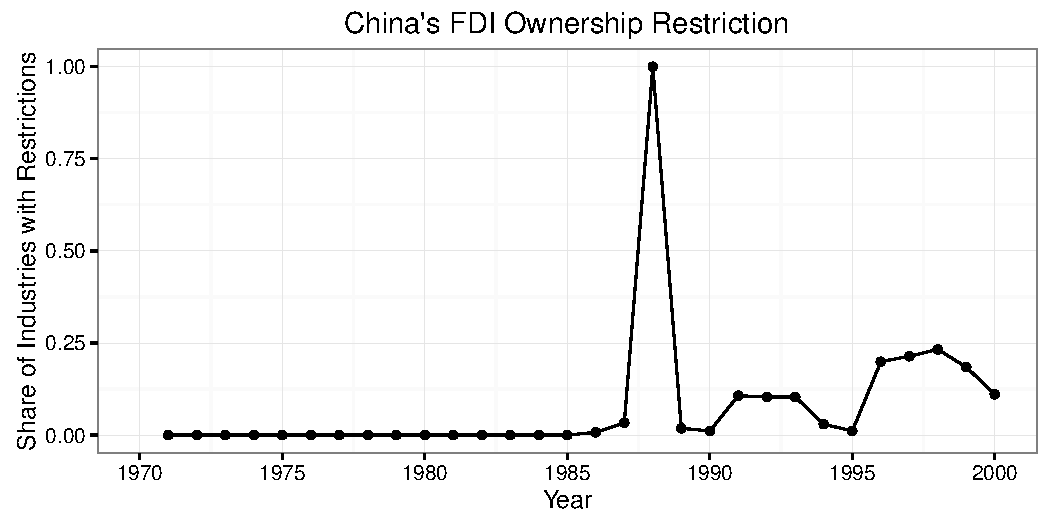
\includegraphics[width=0.75\textwidth,keepaspectratio]{china_fdi_restriction}
\caption{China's FDI Ownership Restriction, as coded in \citet{Pandya2010}.
Prior to 1986, FDI in China was limited to few experimental Special Economic
Zones, and thus not mentioned in US Investment Reports. The sharp spike in 1988
also does not seem to correspond to any actual change in policy, and likely
another artifact of reporting. (See \citet{Zebregs2002} for a historical
overview of China's FDI policy.)}
\label{fig:china_fdi_restriction}
\end{figure}

The two-sided matching model circumvents these thorny measurement issues by
incorporating countries' utility function directly into the model. If we observe
that country $j$ welcomes firms $i_1, i_2, \dots, i_n$ to invest but not others,
we can compare the characteristics of firms $i_1, i_2, \dots i_n$ with the
others to infer country $j$'s preference.


\subsection{Estimating Countries' Preferences for FDI's Technological Intensity}

Laura Alfaro: is all FDI equal? - Use human capital from German firms as a proxy
for all sectors (this works for the OECD sample of that paper, but not more
generally) - Use IPA policy, but this could just be image building by the
country (everyone says that they want advanced manufacturing (cite the picture))

\begin{figure}[!ht] \centering
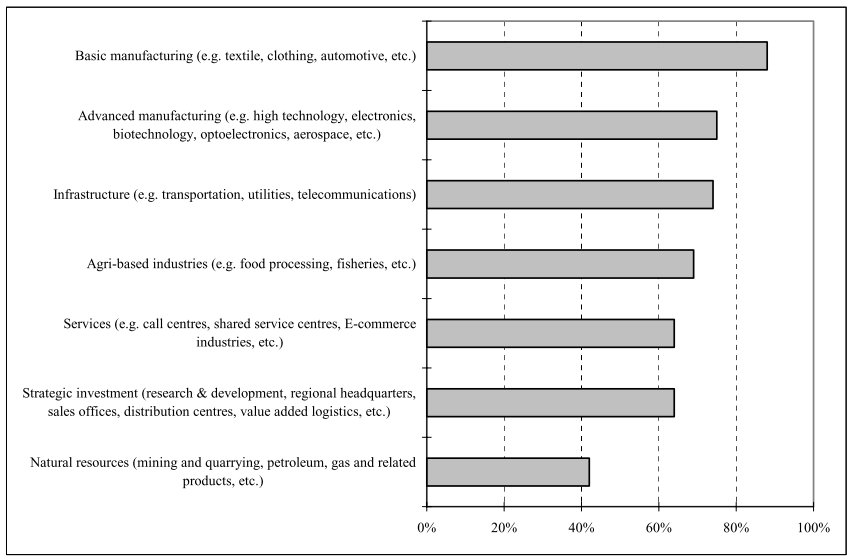
\includegraphics[width=\textwidth,keepaspectratio]{../figure/IPA_target_industries}
  \caption[Target industries by IPA around the world.]{Target industries by IPA around the world. Because of the image
building aspect of investment promotion, almost all IPAs say that they want to
attract ``advanced manufacturing.'' Therefore, using what is listed as
investment priorities may not be a reliable way to measure countries' preference
for FDI. Source: \citet{UNCTAD2001}}
  \label{fig:IPA_target_industries}
\end{figure}

While the political science literature has focused almost exclusively on the
quantity of FDI, treating all FDI as one homogeneous flow of capital, policy
makers seem to pay much more attention to distinguishing types of FDI.
Commenting on the role of International Investment Agreements (IIAs),
\citet{UNCTAD2015} says, ``Today, increasing the quantity of investment is not
enough. What matters is its quality, i.e. the extent to which investment
delivers concrete sustainable development benefits.'' Governments in developing
countries, from Ghana to China, all offer various forms of tax incentives and
fee waivers to attract FDI that invests in a remote region, brings new
technology, or focuses on exporting \citep{Ricupero2000}. Since 2006, China's
official FDI policy has been ``quality over quantity,'' promoting FDI with
intense R\&D in high-productivity sectors \citep{Guangzhou2011}. Indeed, for
developing countries, the hope is that MNCs will transfer their technologies to
the domestic economy by training workers or partnering with local suppliers.

Despite the importance of disaggregating FDI by its quality, data unavailability
remains the bottleneck. The few existing attempts use detailed data from only
one country or limit the sample to OECD countries \citep{Alfaro2003, Alfaro2007,
Javorcik2004}. With cross-country firm level data now available, we often have
information on the firms' industry or even research and development (R\&D)
expenditure. With the two-sided matching model, I will be able to estimate
countries' preferences for firms' technological intensity. I hypothesize that,
since MNCs' technologies takes time to diffuse to local businesses, a country'
preference of high-tech FDI is shaped by its time horizon.

Indeed, we see examples of various kind targeting and FDI policies.

For example, Ireland provides foreign investors with lower tax rate, lower land price, and cash grants for R\&D that do not need to be repaid. China also offers a tax holiday (two years of no tax and three years of half the normal tax rate) in special economic zones to attract more foreign firms \citep{Telford2001}. We see the same widespread use of investment incentives in Southeast Asia \citep{Fletcher2002}. In Vietnam, provincial governments even defy the central government's directive and offer extra-legal incentives to FDI firms \citep{Vu2007}. Not only do these measures not work in attracting more FDI, they also deprive countries of revenues that could be spent on improving the local labor quality and investment climate---factors that are much more conducive to spillover effect and growth.

%%% Local Variables:
%%% mode: latex
%%% TeX-master: "AnhLe_dissertation.tex"
%%% End: